\chapter{The First G-APD Cherenkov Telescope}

The First G-APD Cherenkov Telescope \cite{FACT-Design} (FACT) is a IACT protoype located $\SI{2200}{\metre}$ above sea-level on the Canary island of La Palma.
It measures air-shower-photons with a $\SI{9.5}{\meter\squared}$ aperture provided by a segmented imaging-reflector with $\SI{4.889}{\meter}$ focal-length.
Apart from monitoring bright sources of cosmic gamma-rays, like Markarian 421 and Markarian 501, FACT is used for demonstrating and testing the usage of new technologies in the field of IACTs. Giving it its name, FACT uses a novel kind of detector made of so called Geiger-mode avalanche photomultipliers (GAPD). These photomultipliers make up the 1440 pixels of Silicon-Photo-Multipliers (SiPM), FACT uses to sense photons. Each pixel yields about $\SI{0.1}{\degree}$ field-of-view, giving FACT a total field-of-view of $\SI{4.5}{\degree}$. Using SiPMs instead of Photo-Multiplier-Tubes (PMTs) differentiates FACT from other IACTs and gives it special possibilities. SIPMs are very robust, compared to PMTs and can operate in brighter light. This makes continuos observations even during bright moon possible. The SIPMs furthermore have a high photon detection efficiency. With these assets, FACT is well suited for noticing flares and informing other collaborations of such.
%
\begin{figure}
  \centering
  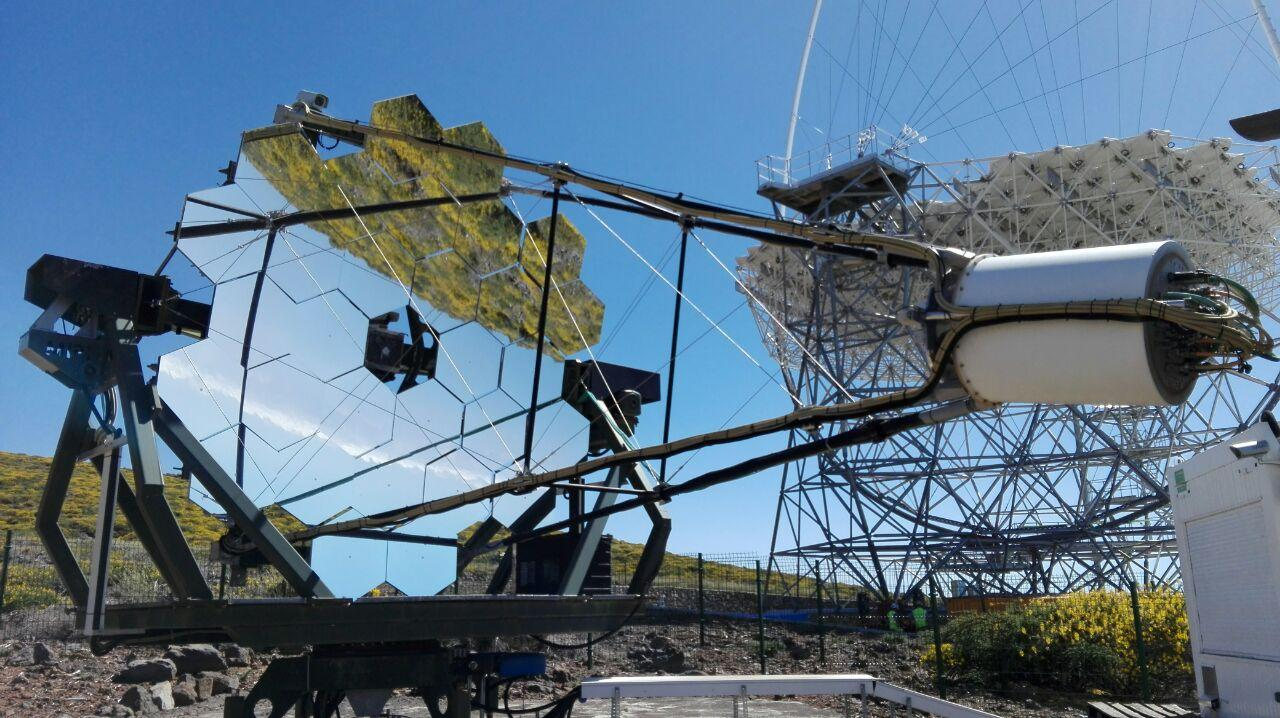
\includegraphics[width=\textwidth]{Plots/fact.jpg}
  \label{fig:fact}
  \caption{The First G-APD Cherenkov Telescope on the Observatory on the Roque des los Muchachos on the island of La Palma. Image by Kevin Schmidt.}
\end{figure}
%
